\documentclass[11pt]{article}

\usepackage[margin=1in]{geometry}
\usepackage{graphicx}
\usepackage{booktabs}
\usepackage{amsmath}
\usepackage{amssymb}
\usepackage{hyperref}
\usepackage{caption}
\usepackage{float}

\title{Conformal Prediction Under Distribution Shift}
\author{Thinh Truong Nguyen}
\date{\today}

\begin{document}
\maketitle

\begin{abstract}
Split-conformal prediction gives regression models finite-sample, distribution-free
prediction intervals with a guaranteed coverage rate, but the guarantee relies on the
calibration and test data being exchangeable. This project asks a direct question:
\emph{what happens to that coverage guarantee when the test distribution no longer
matches the calibration distribution, and what can restore it?} Using synthetic
nonlinear regression data with a known ground-truth function, we build 90\%
split-conformal intervals, confirm they hit their target with no shift, and then
introduce covariate, noise, and subgroup (mixture) shift. Every setting is repeated
over 100 independent calibration/test draws. Coverage falls as low as 18\%. We then
evaluate a range of fixes: recalibration on shifted data, weighted conformal
prediction with exact and estimated likelihood ratios, group-specific calibration,
larger calibration sets, alternative base models, locally adaptive intervals
(normalized scores and conformalized quantile regression), and, for streaming data,
adaptive conformal inference (ACI) and rolling-window calibration. A single theme runs
through the results: every method that restores coverage does so by spending interval
width, and the methods differ mainly in how intelligently they spend it. Recalibration
inflates widths almost sevenfold; weighted conformal stays valid but returns infinite
intervals for most points under strong shift; normalized scores and group-specific
calibration widen intervals only where the data are actually harder; and ACI combined
with a rolling window holds 90\% long-run coverage on drifting streams with no
infinite intervals.
\end{abstract}

\section{Introduction}

Point predictions from a regression model say nothing about how much to trust them.
Conformal prediction addresses this by wrapping any trained model with a procedure
that produces prediction intervals carrying a formal, finite-sample coverage
guarantee: under the sole assumption that calibration and test data are exchangeable
(informally, drawn from the same distribution, in any order), a $(1-\alpha)$
split-conformal interval covers the true outcome at least $(1-\alpha)$ of the time,
regardless of the base model or the data-generating process.

That guarantee is powerful but fragile: it depends entirely on exchangeability. In
real deployments, the data a model sees in production routinely drifts away from
the data it was calibrated on -- new user populations, sensor drift, seasonal
effects, dataset shift between collection sites. When that happens, nothing in the
conformal machinery prevents coverage from silently collapsing. The goal of this
project is to make that failure mode visible, quantify it under controlled synthetic
conditions, and evaluate which fixes restore coverage and at what cost in interval
width.

\section{Background on Conformal Prediction}

Split-conformal prediction (Papadopoulos et al., 2002; Lei et al., 2018) works as
follows for regression:

\begin{enumerate}
  \item Fit a base model $\hat f$ on a training set.
  \item On a separate calibration set of size $n$, compute the nonconformity scores
    $r_i = |y_i - \hat f(x_i)|$, i.e.\ the absolute residuals.
  \item Let $\hat q$ be the $\lceil (n+1)(1-\alpha) \rceil$-th smallest $r_i$. This
    finite-sample correction (rather than the plain $(1-\alpha)$ quantile) is what
    makes the guarantee exact rather than asymptotic. If
    $\lceil (n+1)(1-\alpha) \rceil > n$, the calibration set is too small to certify
    the level and $\hat q = \infty$.
  \item For a new point $x$, output the interval $[\hat f(x) - \hat q,\ \hat f(x) +
    \hat q]$.
\end{enumerate}

\textbf{Coverage guarantee.} If the calibration points and the test point are
exchangeable, then
\[
  1-\alpha \;\le\; \Pr\big(y_{\text{test}} \in [\hat f(x_{\text{test}}) - \hat q,\ \hat f(x_{\text{test}}) + \hat q]\big) \;\le\; 1-\alpha + \frac{1}{n+1},
\]
where the upper bound holds when residuals have no ties. The guarantee is
\emph{marginal} (averaged over the randomness in calibration and test draws, and over
the whole input space), \emph{distribution-free} (no assumption on $\hat f$ or on the
shape of the residual distribution), and holds in finite samples.

\textbf{Where it breaks.} Exchangeability is exactly the assumption that fails under
distribution shift: if the test distribution differs from the calibration
distribution, the calibration residuals $r_i$ are no longer representative of the
residuals the model will make at test time, so $\hat q$ is calibrated to the wrong
error scale. The theorem simply no longer applies. The fixes studied here each recover
some form of the guarantee by changing either \emph{which} residuals are used
(recalibration, group-specific calibration, rolling windows), \emph{how they are
weighted} (weighted conformal), \emph{what the score measures} (normalized scores,
CQR), or \emph{which quantile level is used} (adaptive conformal inference).

\section{Method}

All code is organized into small, single-purpose modules:
\texttt{data\_generation.py} (synthetic data, shift generators, and streams),
\texttt{conformal.py} (offline conformal methods), \texttt{online.py} (online methods
for streams), \texttt{experiments.py} (every experiment below), \texttt{plots.py}
(figures), and \texttt{Main.py}, which reproduces every number and figure in this
report end to end in about three minutes.

The overall pipeline is:

\begin{enumerate}
  \item Generate synthetic $(X, y)$ data from a known nonlinear function
    (Section~\ref{sec:data}).
  \item Train a base regression model once on a training set and hold it fixed, as
    in a deployed system.
  \item Build a 90\% conformal interval from a calibration set.
  \item Evaluate empirical coverage and interval length on test data drawn from the
    same distribution as calibration (Section~\ref{sec:baseline}), and then on test
    data drawn from increasingly shifted distributions (Section~\ref{sec:shift}).
  \item Evaluate fixes (Sections~\ref{sec:fixes}--\ref{sec:online}).
\end{enumerate}

\textbf{Repeated trials.} Split-conformal coverage is itself random: it depends on
which calibration set and which test set were drawn. A single draw can easily land
two percentage points from its expected value, which is the same size as some of the
effects being measured. Every experiment is therefore repeated over 100 independent
trials. In each trial the calibration set and every test set are freshly drawn, and
we report the mean coverage across trials together with its trial-to-trial standard
deviation (sd). The sd describes how far a \emph{single} deployment's coverage can
land from the mean; the standard error of the mean is ten times smaller (about
0.2 percentage points throughout). Figures show $\pm 1$ sd as a shaded band.

\textbf{Paired comparisons.} Within a trial, all methods being compared are scored on
the \emph{same} test set, so differences between methods are not test-draw noise.
All draws are seeded by (experiment, setting, trial), so every number is exactly
reproducible.

Throughout, the target coverage is $1-\alpha = 90\%$ ($\alpha = 0.10$). ``Coverage''
is the fraction of test points whose true $y$ falls inside its interval, and
``interval length'' is upper minus lower bound ($2\hat q$ for symmetric intervals).

\section{Synthetic Data Setup}
\label{sec:data}

Ground truth is known because the data are generated by us. Each input
$x = (x_0, x_1, x_2, x_3)$ is drawn i.i.d.\ from $\mathcal N(x_{\text{loc}},
x_{\text{scale}}^2)$, and the target is
\[
  y = 2x_0 - 1.5x_1 + 0.8x_2^2 + \sin(2x_3) + \varepsilon, \qquad
  \varepsilon \sim \mathcal N(0, \text{noise\_std}^2).
\]
The quadratic and sinusoidal terms make the relationship nonlinear, so a base model
has to learn structure rather than fit a straight line; a random forest (300 trees)
is the default base model except in the model-comparison experiment
(Section~\ref{sec:models}).

Baseline (unshifted) settings are $x_{\text{loc}} = 0$, $x_{\text{scale}} = 1$,
$\text{noise\_std} = 1$. Data set sizes are 1500 training points, 500 calibration
points, and 1000 test points, unless an experiment explicitly varies one of these.

Three kinds of shift are used, each isolating a different real-world failure mode:

\begin{itemize}
  \item \textbf{Covariate shift}: increase $x_{\text{loc}}$ from 0 to 3, moving test
    inputs into a region the model saw little or no training data for.
  \item \textbf{Noise shift}: increase $\text{noise\_std}$ from 1 to 3, keeping
    inputs in-distribution but making the labels themselves noisier.
  \item \textbf{Subgroup (mixture) shift}: the population is a mixture of a
    low-noise group A ($\text{noise\_std}=1.0$) and a high-noise group B
    ($\text{noise\_std}=2.5$). Calibration data come from a mixture with 20\% group B;
    at test time the share of group B rises to 80\%, while each group's own
    conditional distribution never changes. Both groups have identical input
    distributions, so group membership is \emph{not} visible in $x$.
\end{itemize}

Two further variants support the adaptive-method experiments:

\begin{itemize}
  \item \textbf{Heteroscedastic data} (Section~\ref{sec:adaptive}): the noise standard
    deviation depends on the inputs, $\text{sd}(\varepsilon \mid x) = 0.2 + |x_3|$,
    so the difficulty of a point \emph{is} visible in $x$. Shift is introduced by
    moving only the mean of $x_3$, which pushes test points toward the noisy region.
  \item \textbf{Streams} (Section~\ref{sec:online}): points arrive one at a time and
    $x_{\text{loc}}$ and $\text{noise\_std}$ change over time.
\end{itemize}

\section{Baseline Experiment}
\label{sec:baseline}

With no shift, the random forest is calibrated at the nominal 90\% level. A single
illustrative draw gives:

\begin{center}
\begin{tabular}{lr}
\toprule
Quantity & Value \\
\midrule
Target coverage & 90.0\% \\
Conformal half-width $\hat q$ & 2.096 \\
Empirical coverage (single draw) & 92.2\% \\
Interval length & 4.192 \\
\midrule
Empirical coverage (mean $\pm$ sd over 100 trials) & 90.0\% $\pm$ 1.6\% \\
\bottomrule
\end{tabular}
\end{center}

\begin{figure}[H]
  \centering
  \includegraphics[width=0.75\linewidth]{results/baseline.png}
  \caption{Predicted vs.\ actual $y$ on one unshifted test set. The shaded band is
  the $\pm \hat q$ conformal band around perfect prediction; blue points fall inside
  their interval, red crosses do not.}
  \label{fig:baseline}
\end{figure}

The single draw lands at 92.2\%, but this is sampling noise rather than a systematic
effect: averaged over 100 trials, coverage is 90.0\%, inside the theoretical range
$[90.0\%, 90.2\%]$ given by the bound above with $n=500$. The trial-to-trial sd of
1.6 percentage points is close to what theory predicts. Conditional on the
calibration set, coverage follows a Beta distribution with variance about
$\alpha(1-\alpha)/(n+2)$, giving an sd of 1.3 points. Test-set sampling adds a binomial
sd of $\sqrt{0.09/1000} \approx 0.9$ points. Together these give about 1.6 points.

\section{Distribution-Shift Experiments}
\label{sec:shift}

\subsection{Covariate shift}

\begin{figure}[H]
  \centering
  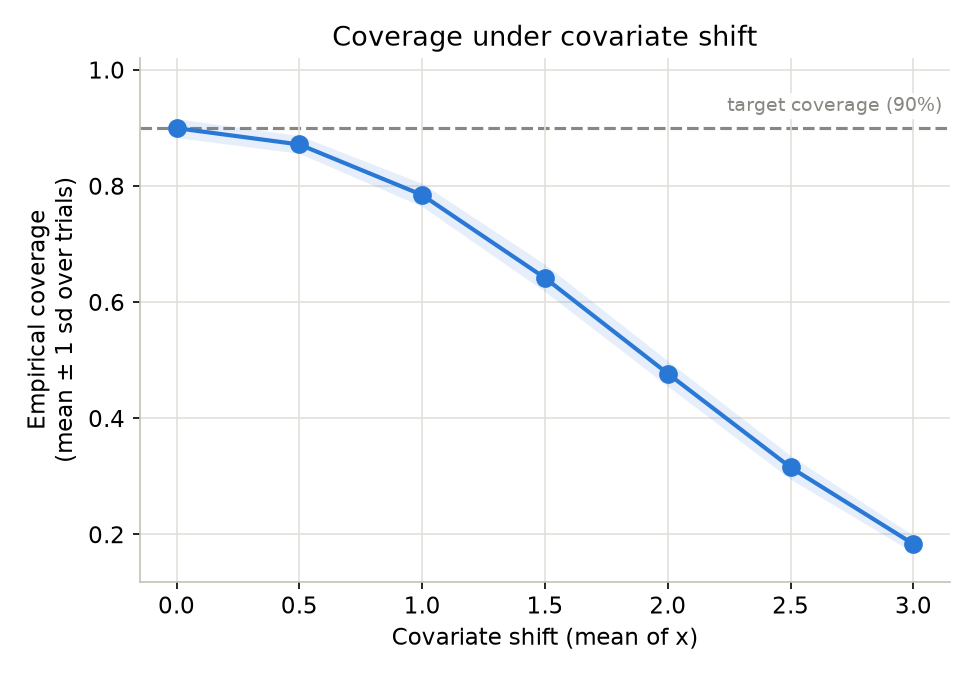
\includegraphics[width=0.7\linewidth]{results/covariate_shift.png}
  \caption{Empirical coverage as the test input mean $x_{\text{loc}}$ moves from 0 to
  3, using intervals calibrated at $x_{\text{loc}}=0$. Shaded: $\pm 1$ sd over 100
  trials.}
  \label{fig:covariate_shift}
\end{figure}

\begin{center}
\begin{tabular}{rrr}
\toprule
Shift ($x_{\text{loc}}$) & Coverage (mean $\pm$ sd) & Interval length \\
\midrule
0.0 & 90.0\% $\pm$ 1.6 & 4.06 \\
1.0 & 78.5\% $\pm$ 2.0 & 4.06 \\
2.0 & 47.7\% $\pm$ 2.2 & 4.06 \\
3.0 & 18.4\% $\pm$ 1.5 & 4.06 \\
\bottomrule
\end{tabular}
\end{center}

Coverage collapses from 90\% to under one-fifth as inputs move away from the
training region. The interval length never changes because it is fixed at
calibration time. The model's predictions, however, become increasingly biased on
inputs it has not seen: a random forest cannot extrapolate the linear $2x_0 - 1.5x_1$
trend or the growing $0.8x_2^2$ term beyond its training range. A fixed-width band
around a biased prediction misses the truth far more often.

\subsection{Noise shift}

\begin{figure}[H]
  \centering
  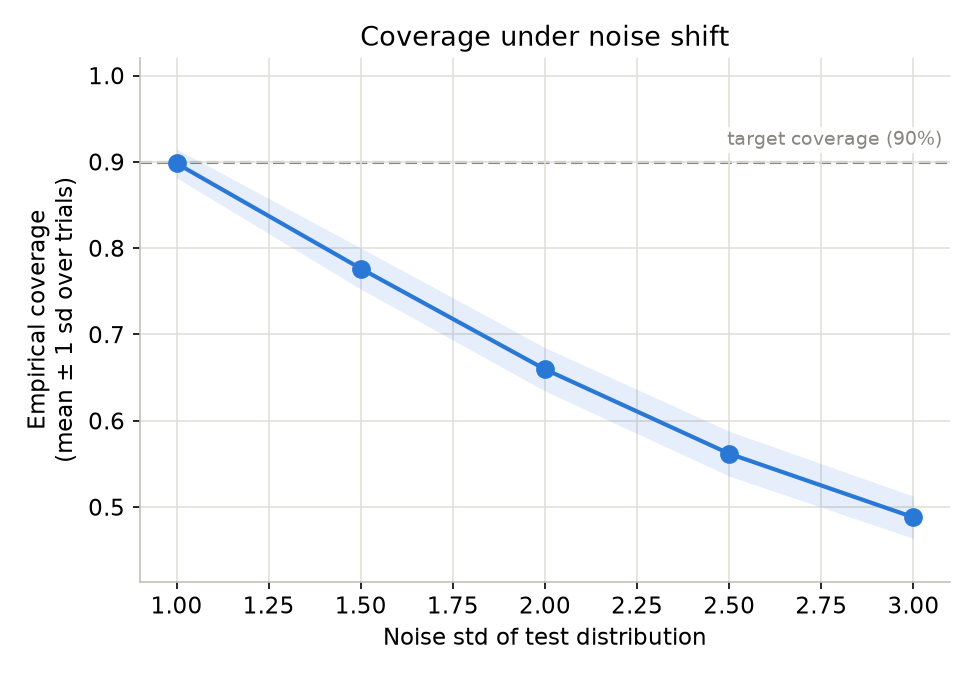
\includegraphics[width=0.7\linewidth]{results/noise_shift.png}
  \caption{Empirical coverage as the test-label noise std grows from 1 to 3, with
  inputs kept in-distribution.}
  \label{fig:noise_shift}
\end{figure}

\begin{center}
\begin{tabular}{rrr}
\toprule
Noise std & Coverage (mean $\pm$ sd) & Interval length \\
\midrule
1.0 & 89.8\% $\pm$ 1.7 & 4.06 \\
2.0 & 66.0\% $\pm$ 2.5 & 4.06 \\
3.0 & 48.8\% $\pm$ 2.4 & 4.06 \\
\bottomrule
\end{tabular}
\end{center}

Even with inputs fully in-distribution, coverage fails once the intrinsic label noise
at test time exceeds what calibration prepared for. The calibrated width is simply
not wide enough for the new noise level.

\subsection{Subgroup shift}

\begin{figure}[H]
  \centering
  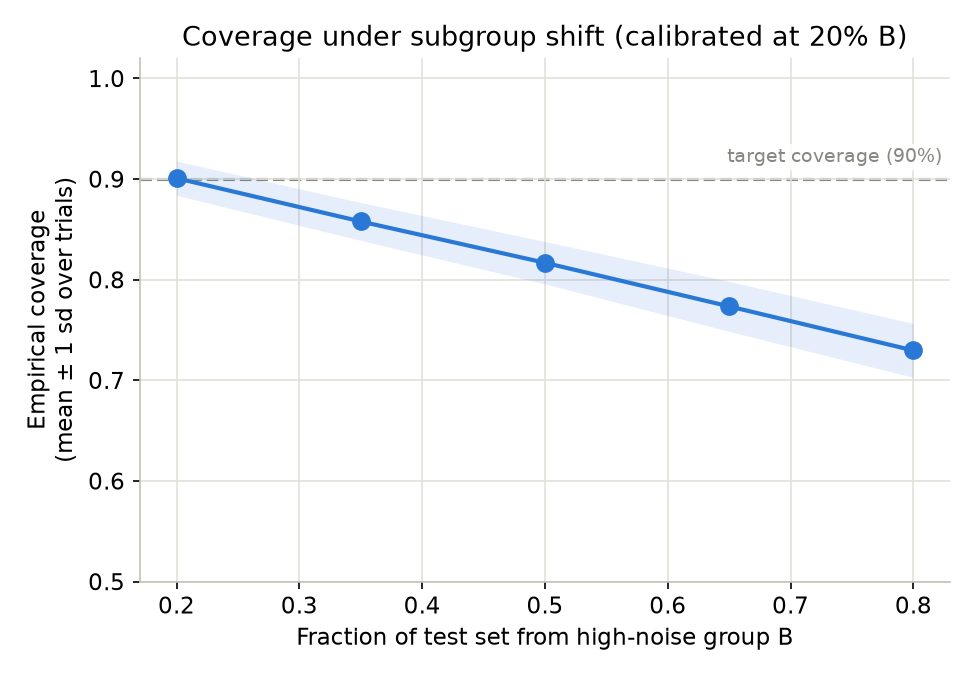
\includegraphics[width=0.7\linewidth]{results/subgroup_shift.png}
  \caption{Empirical coverage as the fraction of high-noise group B in the test
  population grows, using a single pooled width calibrated on the baseline mixture
  (20\% group B).}
  \label{fig:subgroup_shift}
\end{figure}

\begin{center}
\begin{tabular}{rrr}
\toprule
Fraction group B & Coverage (mean $\pm$ sd) & Interval length \\
\midrule
0.20 (no shift) & 90.1\% $\pm$ 1.7 & 5.13 \\
0.50 & 81.7\% $\pm$ 2.1 & 5.13 \\
0.80 & 73.0\% $\pm$ 2.7 & 5.13 \\
\bottomrule
\end{tabular}
\end{center}

Because calibration uses the baseline 20\% mixture, coverage is on target when the
test population matches it. As the share of group B grows, coverage falls linearly
to 73.0\%. The pooled width is a compromise: wider than group A needs and narrower
than group B needs. It hits 90\% only for the particular mixture it was tuned to.
Each group's conditional distribution never changes; only the mix does.

\section{Fixes for Offline Shift}
\label{sec:fixes}

\subsection{Recalibration}

If we can draw a fresh, \emph{labeled} calibration set from the shifted distribution
itself and recompute $\hat q$, coverage is restored by construction, because
calibration and test data are exchangeable again. The open question is the cost.
Results for this fix and the next are shown together in Figure~\ref{fig:fixes_covariate}
and the table in Section~\ref{sec:weighted}.

Recalibrated coverage stays at 89.8--90.1\% at every shift level. But the median
interval length grows from 4.08 to \textbf{27.65}, a 6.8-fold increase.
Recalibration does not make the model better at the shifted task; it correctly
admits that the model's predictions are far less reliable there, and widens the
interval enough to compensate. Reporting coverage alone would make this look like a
clean fix. Reporting width alongside it reveals that the ``fix'' is really honest
uncertainty quantification of a model operating far outside its competence. It also
requires labeled data from the new distribution, which a real deployment usually
does not have at the moment of shift.

\subsection{Weighted conformal prediction}
\label{sec:weighted}

Weighted conformal prediction (Tibshirani et al., 2019) handles covariate shift
\emph{without} new labels. If only the input distribution changes, from
$P_{\text{cal}}(x)$ to $P_{\text{test}}(x)$, and $P(y \mid x)$ stays the same, each
calibration residual can be reweighted by the likelihood ratio
$w(x) = dP_{\text{test}}(x)/dP_{\text{cal}}(x)$. For a test point $x$, $\hat q(x)$ is
the $(1-\alpha)$ quantile of the weighted distribution
\[
  \sum_{i=1}^n p_i(x)\, \delta_{r_i} + p_{n+1}(x)\, \delta_{+\infty},
  \qquad
  p_i(x) = \frac{w(x_i)}{\sum_{j} w(x_j) + w(x)},\quad
  p_{n+1}(x) = \frac{w(x)}{\sum_{j} w(x_j) + w(x)},
\]
which restores the $1-\alpha$ coverage guarantee when $w$ is correct. The point mass
at $+\infty$ matters. If the test point's own weight $p_{n+1}(x)$ exceeds $\alpha$,
the quantile lands on $+\infty$ and the interval is infinite.

Two versions are compared, both using the original \emph{unshifted} calibration set:
\begin{itemize}
  \item \textbf{Exact weights}: the true ratio of the two Gaussians,
    $\log w(x) = \mu^\top x - \tfrac12\|\mu\|^2$ with $\mu = x_{\text{loc}}\mathbf 1$.
  \item \textbf{Estimated weights}: a logistic regression trained to distinguish
    1000 unlabeled source inputs from 1000 unlabeled shifted inputs; the odds give
    $\hat w(x)$. Logistic regression is well-specified here because the true
    log-ratio is linear in $x$. The classifier is fit on data separate from the
    calibration set.
\end{itemize}

\begin{figure}[H]
  \centering
  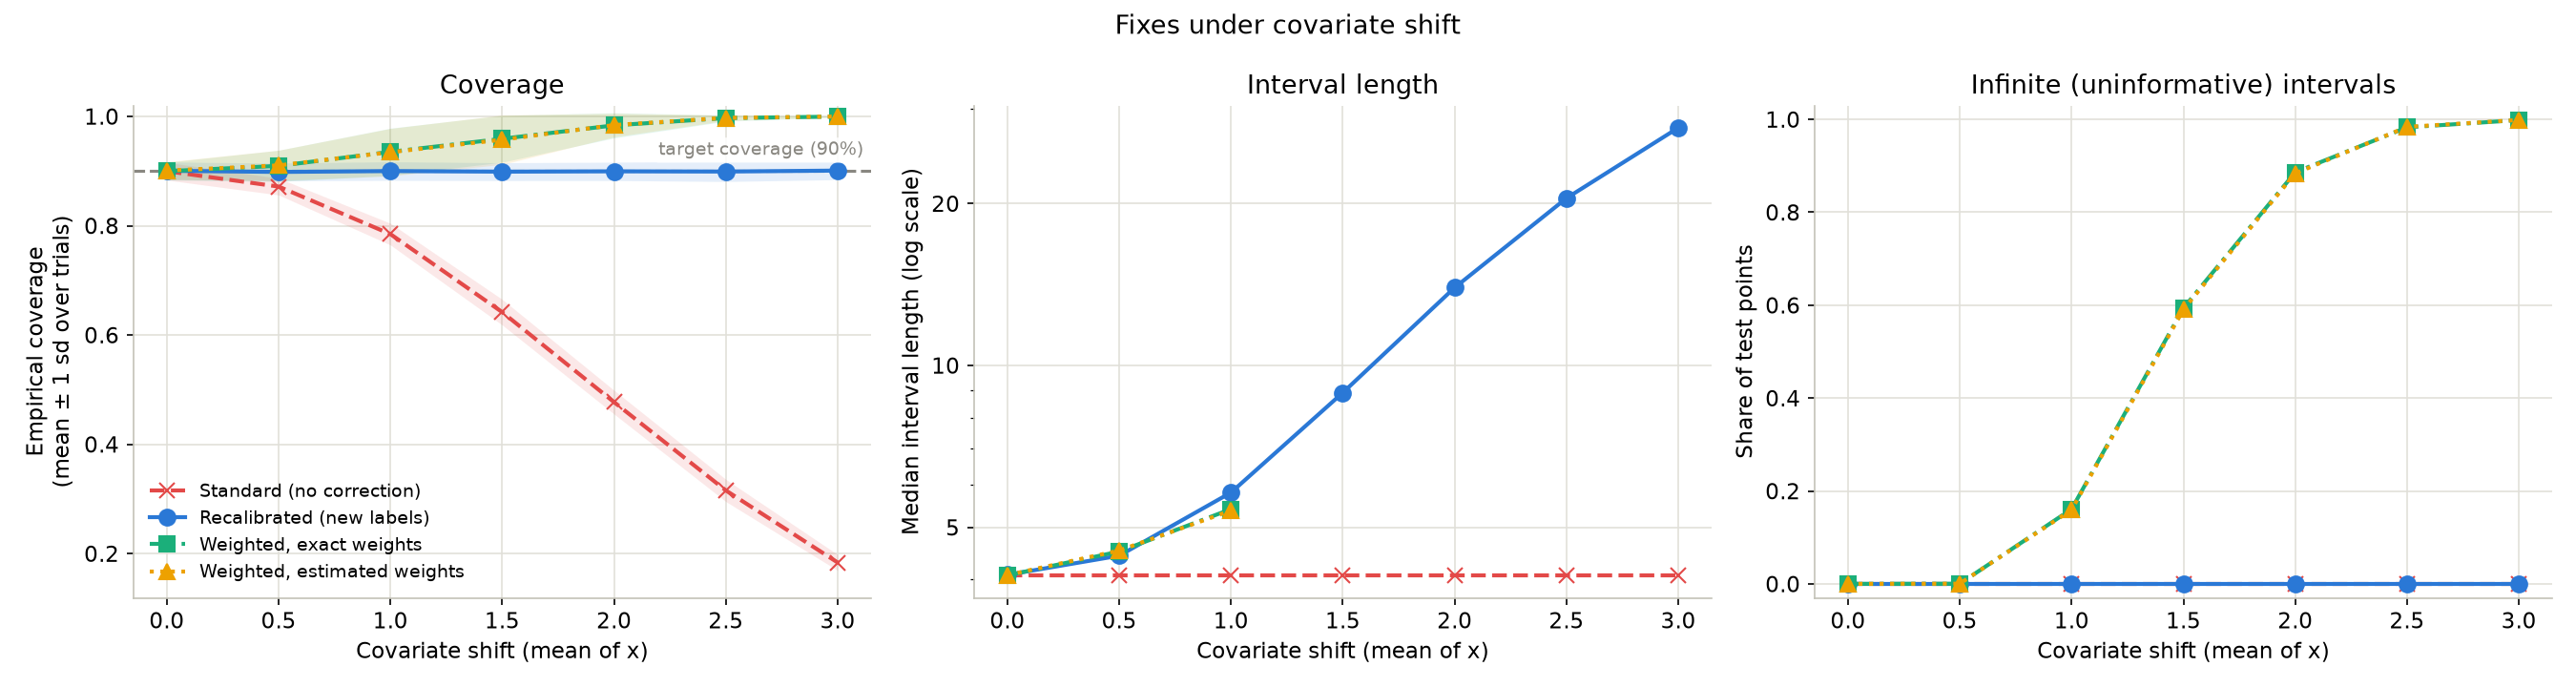
\includegraphics[width=\linewidth]{results/fixes_covariate.png}
  \caption{Fixes under covariate shift, all scored on the same test sets. Left:
  coverage ($\pm 1$ sd). Middle: median interval length (log scale); weighted
  methods drop off the plot once more than half their intervals are infinite.
  Right: share of test points that received an infinite interval.}
  \label{fig:fixes_covariate}
\end{figure}

\begin{center}
\small
\begin{tabular}{r r rr rrr rr}
\toprule
 & Standard & \multicolumn{2}{c}{Recalibrated} & \multicolumn{3}{c}{Weighted (exact)} & \multicolumn{2}{c}{Weighted (estimated)} \\
\cmidrule(lr){2-2}\cmidrule(lr){3-4}\cmidrule(lr){5-7}\cmidrule(lr){8-9}
Shift & Cov. & Cov. & Length & Cov. & Length & \% inf & Cov. & \% inf \\
\midrule
0.0 & 90.0\% & 90.0\% & 4.08 & 90.0\% & 4.07 & 0\% & 90.1\% & 0\% \\
0.5 & 87.2\% & 89.8\% & 4.43 & 90.9\% & 4.51 & 0\% & 91.0\% & 0\% \\
1.0 & 78.5\% & 90.0\% & 5.80 & 93.5\% & 5.40 & 16\% & 93.4\% & 16\% \\
1.5 & 64.2\% & 89.9\% & 8.90 & 95.9\% & $\infty$ & 59\% & 95.7\% & 59\% \\
2.0 & 47.7\% & 89.9\% & 13.95 & 98.4\% & $\infty$ & 89\% & 98.4\% & 88\% \\
3.0 & 18.4\% & 90.1\% & 27.65 & 100.0\% & $\infty$ & 100\% & 100.0\% & 100\% \\
\bottomrule
\end{tabular}
\end{center}

\noindent(Lengths are medians over test points; ``\% inf'' is the share of
infinite intervals.)

Weighted conformal does what the theory promises: coverage never falls below target,
and it needs no labels from the shifted distribution. At mild shift ($x_{\text{loc}}
= 0.5$) it matches recalibration almost exactly. Estimated weights perform almost
identically to exact ones, so in this setting the cost of not knowing the shift is
negligible.

Beyond mild shift, however, a growing share of intervals is infinite: 16\% at
$x_{\text{loc}}=1$, 59\% at 1.5, and essentially all at 2.5 and above. The cause is
weight degeneracy. For two unit-variance Gaussians in $d=4$ dimensions,
$\mathbb E_{\text{cal}}[w^2] = e^{\|\mu\|^2} = e^{4 x_{\text{loc}}^2}$, so the
\emph{effective sample size} $(\sum w_i)^2 / \sum w_i^2$ of the calibration set is
roughly $n e^{-4x_{\text{loc}}^2}$: about 180 at shift 0.5, about 9 at shift 1, and
below 1 from shift 1.5 on. Only a handful of calibration points resemble the shifted test
points, so the method cannot certify any finite quantile and returns $(-\infty,
\infty)$. This is the honest answer, since the calibration data contain almost no
information about the shifted region. In practice weighted conformal is a fix for
\emph{moderate} covariate shift, where source and target overlap substantially. Its
coverage above target at larger shifts comes from those infinite intervals, not from
useful ones.

\subsection{Group-specific calibration}

For the subgroup-mixture setting, we calibrate on the baseline mixture (20\% group B)
and compute both a pooled width and one width per group. Averaged over trials, the
per-group half-widths are A: 2.04 and B: 4.28, versus pooled: 2.57. We then evaluate
both as the test-set mixture shifts toward group B.

\begin{figure}[H]
  \centering
  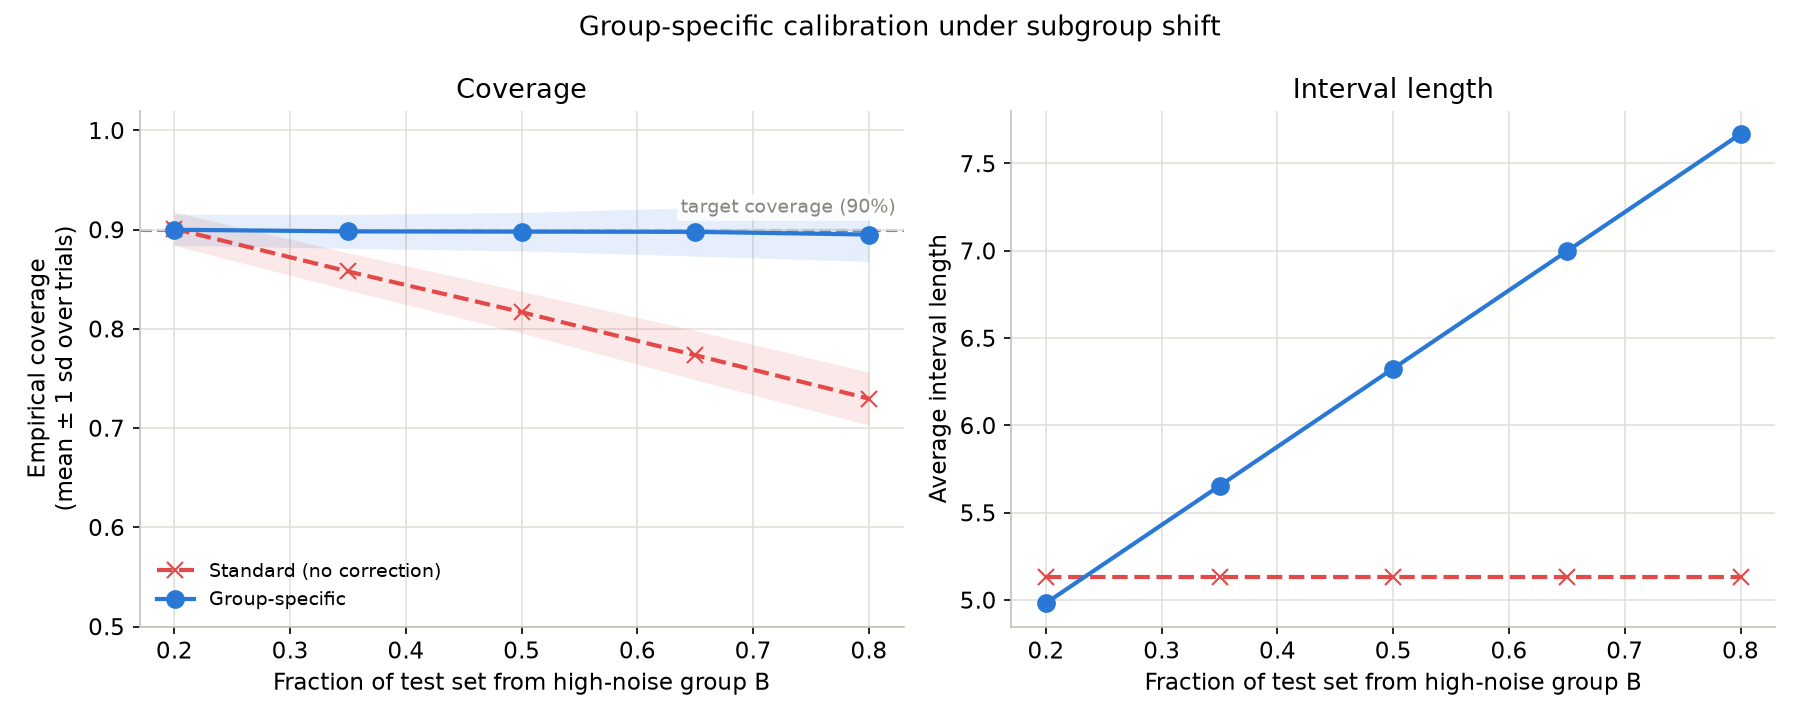
\includegraphics[width=0.95\linewidth]{results/fixes_subgroup.png}
  \caption{Standard (pooled) vs.\ group-specific calibration as the test population's
  group-B fraction grows from its calibration-time value (20\%) to 80\%. Left:
  coverage ($\pm 1$ sd). Right: average interval length.}
  \label{fig:fixes_subgroup}
\end{figure}

\begin{center}
\small
\begin{tabular}{rrrrr}
\toprule
Frac.\ group B & Cov.\ (pooled) & Length (pooled) & Cov.\ (group-specific) & Length (group-specific) \\
\midrule
0.20 & 90.1\% & 5.13 & 90.0\% & 4.98 \\
0.50 & 81.7\% & 5.13 & 89.8\% & 6.33 \\
0.80 & 73.0\% & 5.13 & 89.5\% & 7.67 \\
\bottomrule
\end{tabular}
\end{center}

At the calibration-time mixture, pooled and group-specific calibration agree, and
group-specific intervals are even slightly shorter on average. As the mixture shifts,
pooled coverage drops to 73.0\%, while group-specific coverage stays at 89.5--90.0\%.
Each test point is scored against \emph{its own group's} width, and each group's
conditional noise level never changed. The average length grows only because more
test points belong to the group that genuinely needs wider intervals. This is the
cleanest fix in the project, but it requires knowing group membership at both
calibration and test time (see Section~\ref{sec:limitations}).

\subsection{Calibration set size}

Does a larger calibration set, drawn from the shifted distribution at covariate shift
$=2.0$, make recalibration more reliable? In each of 100 trials we draw a fresh test
set and a fresh calibration set of each size.

\begin{figure}[H]
  \centering
  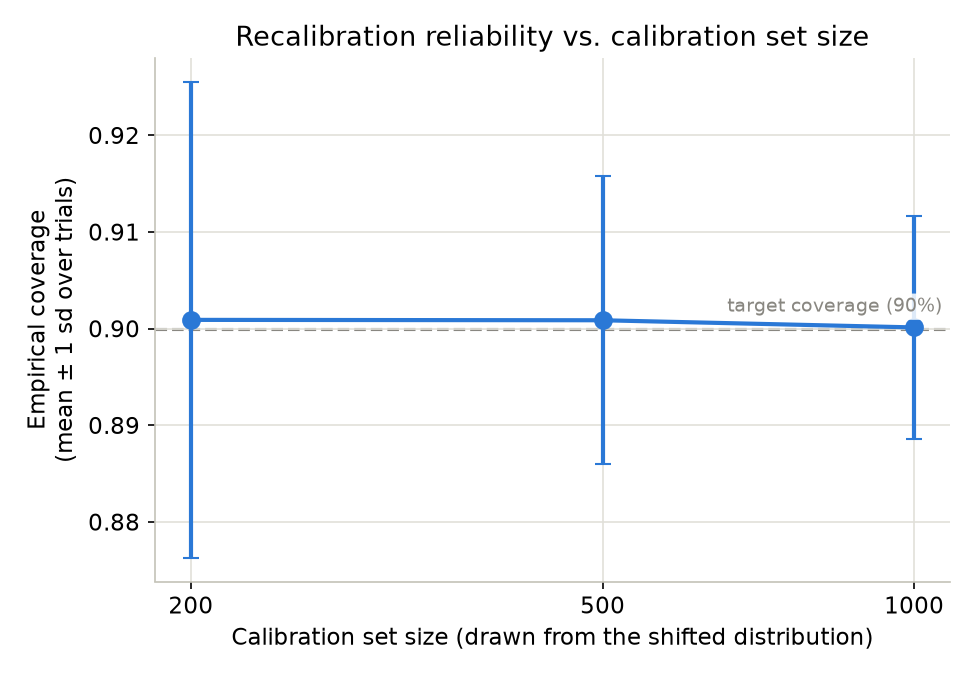
\includegraphics[width=0.7\linewidth]{results/calibration_size.png}
  \caption{Mean coverage ($\pm 1$ sd over 100 trials) after recalibrating with
  calibration sets of size 200, 500, and 1000 drawn from the shifted distribution.}
  \label{fig:calibration_size}
\end{figure}

\begin{center}
\begin{tabular}{rrrrr}
\toprule
Calib.\ size & Mean coverage & Sd coverage & Mean length & Sd length \\
\midrule
200 & 90.1\% & 2.5pp & 14.06 & 1.32 \\
500 & 90.1\% & 1.5pp & 13.95 & 0.84 \\
1000 & 90.0\% & 1.2pp & 13.87 & 0.57 \\
\bottomrule
\end{tabular}
\end{center}

The \emph{mean} coverage is on target at every size: even 200 points recalibrate
correctly on average. What changes is \emph{reliability}. The sd of achieved
coverage shrinks from 2.5 to 1.2 percentage points, closely matching the theoretical
values (2.3, 1.6 and 1.3 points from the Beta-plus-binomial calculation in
Section~\ref{sec:baseline}). The remaining 1.2 points at $n=1000$ is mostly test-set
sampling noise, which no calibration set can remove. In a real deployment only one
calibration set is drawn, so this variance is exactly the risk of an unlucky draw
silently under-covering. A larger calibration set buys protection against that, not a
better average.

\subsection{Does the choice of base model matter?}
\label{sec:models}

We compare linear regression, random forest, and gradient boosting, all trained on
the same data and conformalized on the same calibration draws, under noise shift.

\begin{figure}[H]
  \centering
  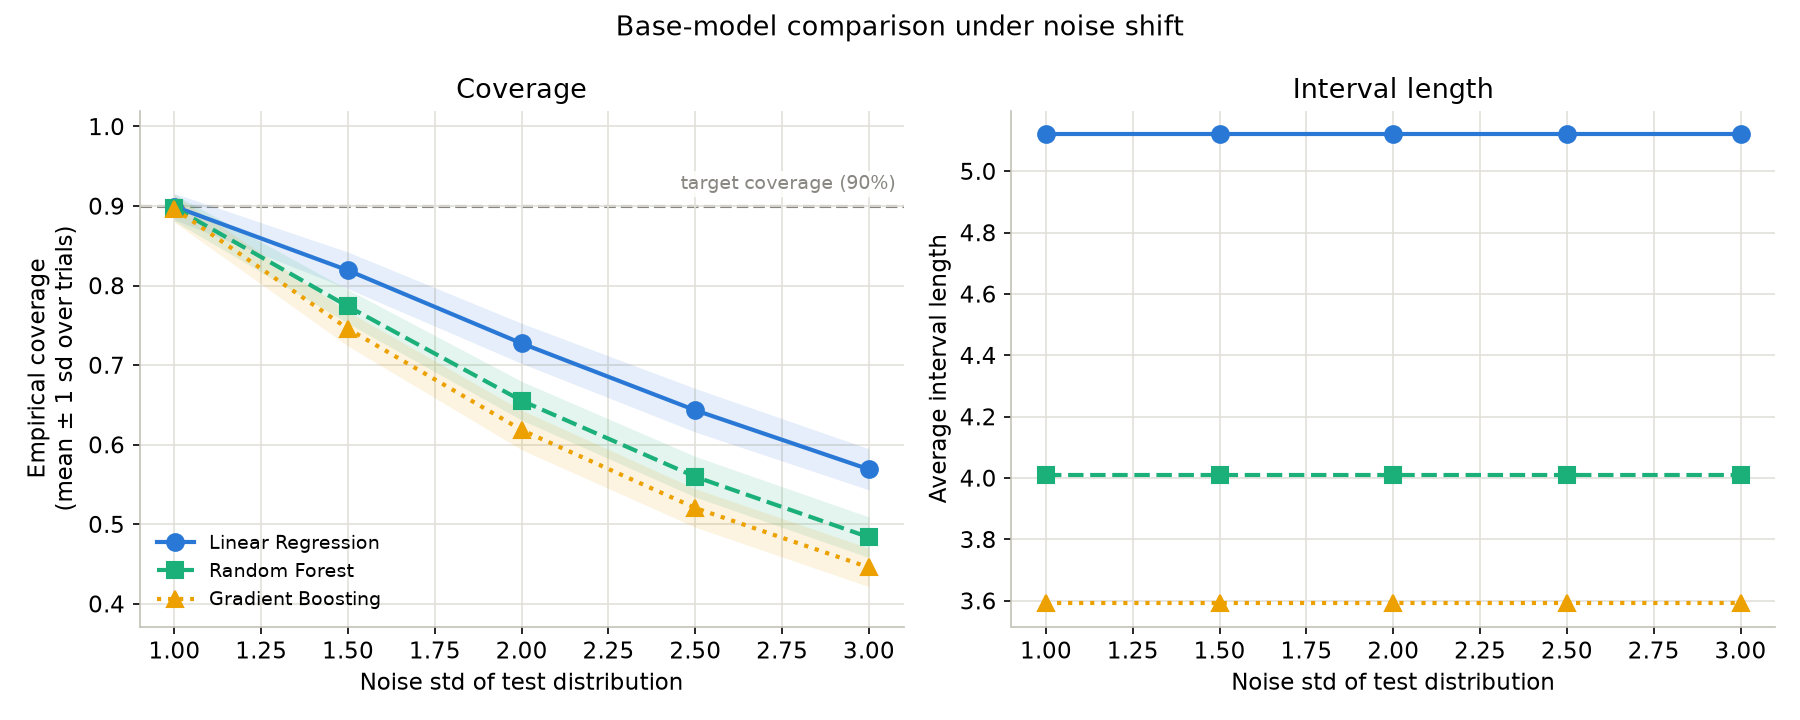
\includegraphics[width=0.95\linewidth]{results/method_comparison.png}
  \caption{Left: coverage under noise shift for three base models ($\pm 1$ sd).
  Right: their (constant, calibration-time) interval lengths.}
  \label{fig:method_comparison}
\end{figure}

\begin{center}
\begin{tabular}{lrrr}
\toprule
Model & Coverage @ noise=1.0 & Coverage @ noise=3.0 & Length (constant) \\
\midrule
Linear Regression & 89.9\% & 56.9\% & 5.12 \\
Random Forest & 89.8\% & 48.4\% & 4.01 \\
Gradient Boosting & 89.7\% & 44.6\% & 3.59 \\
\bottomrule
\end{tabular}
\end{center}

All three models are on target without shift and all degrade under shift: coverage
failure is a property of the exchangeability assumption, not of any particular model.
The ranking under shift is the reverse of the ranking in accuracy, and the reason is
instructive. Linear regression cannot represent the quadratic and sinusoidal terms,
so its residuals contain a large, fixed \emph{approximation error} on top of the
noise, and its interval is correspondingly wider. When noise grows, that fixed error
makes up a shrinking share of the residual, and the extra slack in the wider interval
absorbs part of the increase. Gradient boosting's residuals are almost pure noise, so
its tight interval has no slack, and every increase in noise turns directly into lost
coverage. A more accurate model buys narrower intervals in-distribution, but no
robustness to shift.

\section{Locally Adaptive Intervals}
\label{sec:adaptive}

Every interval so far has had the same width everywhere in the input space. When
difficulty varies with $x$, a fixed width is a compromise: too wide where the data
are easy and too narrow where they are hard. The guarantee is only \emph{marginal},
so that compromise can still average to 90\%. But it becomes a liability under shift:
any shift that moves test points toward the hard region breaks coverage, as in the
subgroup experiment.

We compare three methods on heteroscedastic data, $\text{sd}(\varepsilon \mid x) =
0.2 + |x_3|$:

\begin{itemize}
  \item \textbf{Standard}: fixed-width split conformal with score $|y - \hat f(x)|$.
  \item \textbf{Normalized scores} (locally weighted conformal; Lei et al., 2018):
    score $|y - \hat f(x)| / \hat\sigma(x)$, interval $\hat f(x) \pm \hat q\,
    \hat\sigma(x)$. Here $\hat\sigma$ is a random forest (minimum leaf size 20) fit to
    the absolute \emph{out-of-bag} residuals of $\hat f$ on the training set. Using
    out-of-bag residuals gives it honest residuals rather than the overfit in-sample
    ones.
  \item \textbf{Conformalized quantile regression (CQR)} (Romano et al., 2019):
    gradient-boosted quantile regressors $\hat q_{\text{lo}}, \hat q_{\text{hi}}$ at
    levels 5\% and 95\%, score $\max(\hat q_{\text{lo}}(x) - y,\ y - \hat
    q_{\text{hi}}(x))$, interval $[\hat q_{\text{lo}}(x) - \hat q,\ \hat
    q_{\text{hi}}(x) + \hat q]$.
\end{itemize}

\begin{figure}[H]
  \centering
  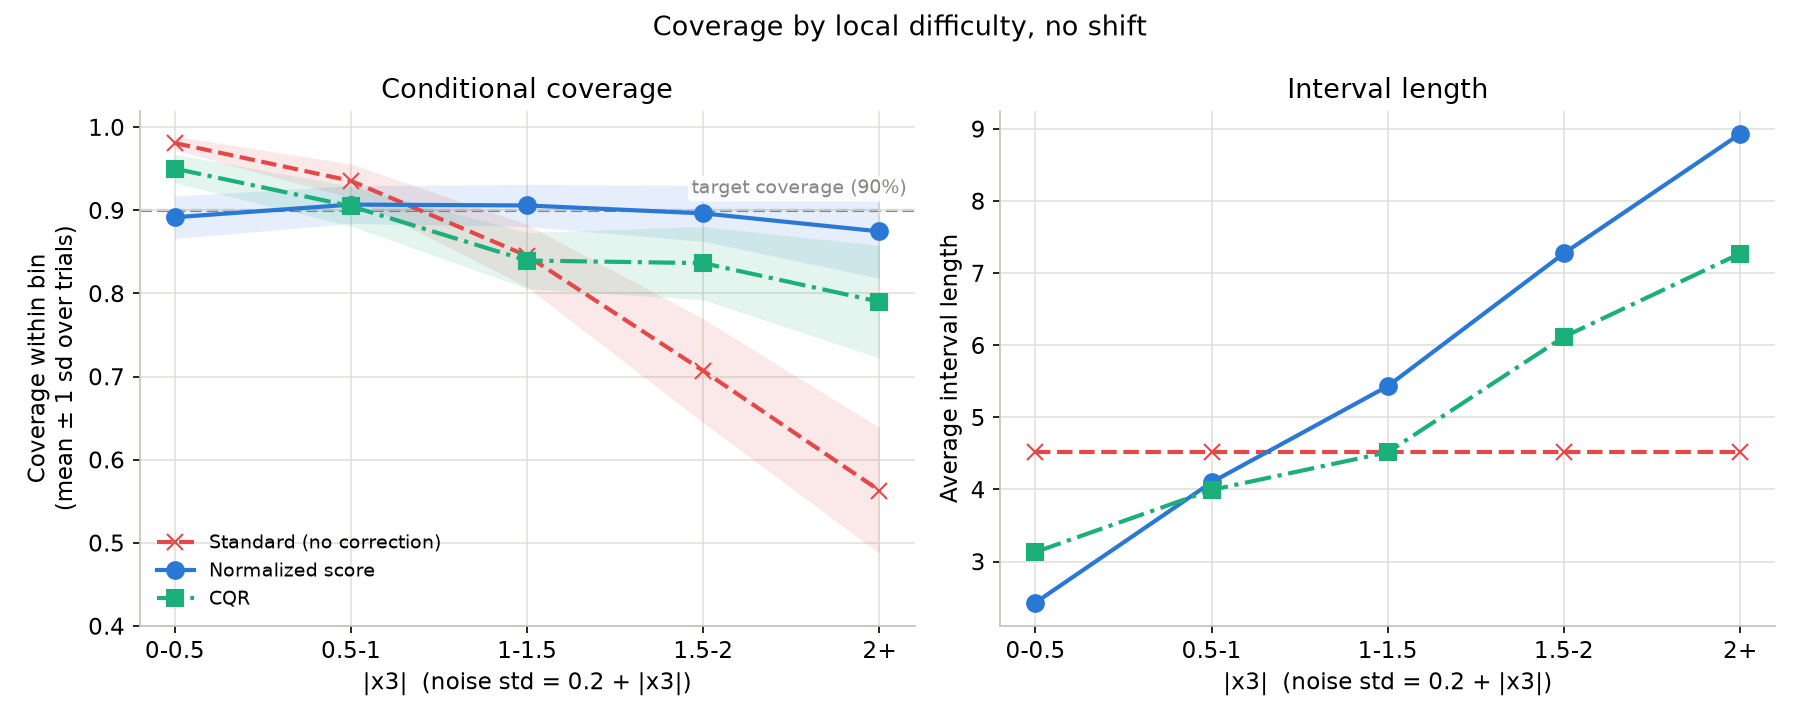
\includegraphics[width=0.95\linewidth]{results/adaptive_conditional.png}
  \caption{No shift: coverage and interval length within bins of $|x_3|$, the driver
  of the noise level. All three methods have 90\% marginal coverage.}
  \label{fig:adaptive_conditional}
\end{figure}

\begin{center}
\begin{tabular}{l rr rr rr}
\toprule
 & \multicolumn{2}{c}{Standard} & \multicolumn{2}{c}{Normalized} & \multicolumn{2}{c}{CQR} \\
\cmidrule(lr){2-3}\cmidrule(lr){4-5}\cmidrule(lr){6-7}
$|x_3|$ & Cov. & Length & Cov. & Length & Cov. & Length \\
\midrule
0--0.5 & 98.1\% & 4.51 & 89.2\% & 2.43 & 95.0\% & 3.13 \\
0.5--1 & 93.5\% & 4.51 & 90.7\% & 4.10 & 90.5\% & 3.99 \\
1--1.5 & 84.5\% & 4.51 & 90.6\% & 5.43 & 84.0\% & 4.52 \\
1.5--2 & 70.7\% & 4.51 & 89.6\% & 7.27 & 83.6\% & 6.12 \\
2+ & 56.3\% & 4.51 & 87.5\% & 8.93 & 79.0\% & 7.27 \\
\bottomrule
\end{tabular}
\end{center}

Even with no shift, the standard method's 90\% is an average of 98\% in the easy
region and 56\% in the hardest one. Normalized scores give close to 90\% in every
bin, using short intervals where the data are easy and long ones where they are
hard. CQR moves in the right direction but under-covers the noisy tail.

\begin{figure}[H]
  \centering
  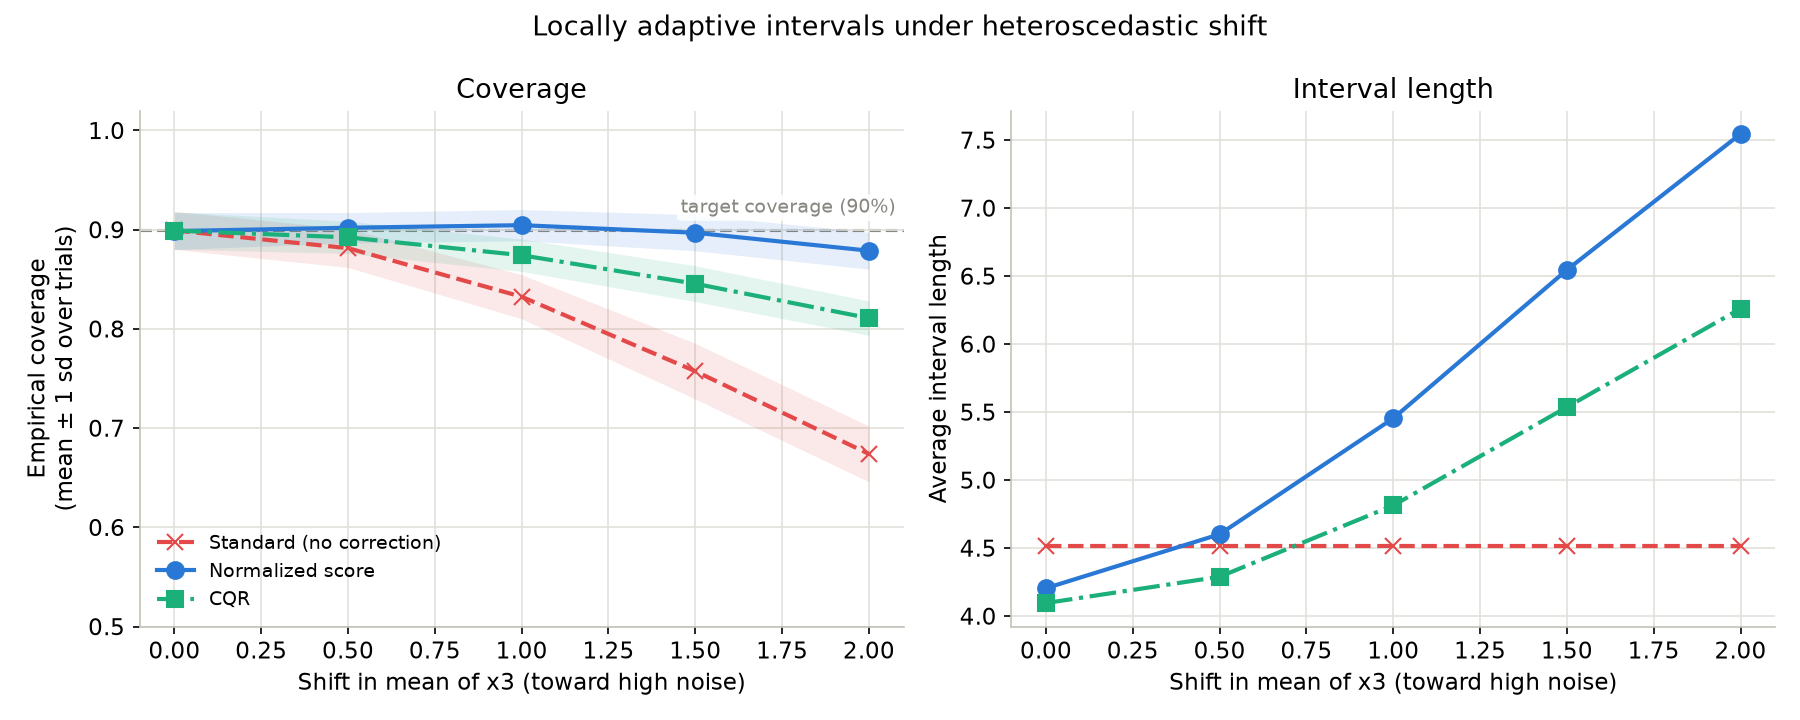
\includegraphics[width=0.95\linewidth]{results/adaptive_shift.png}
  \caption{Coverage ($\pm 1$ sd) and average interval length as the mean of $x_3$
  shifts toward the high-noise region.}
  \label{fig:adaptive_shift}
\end{figure}

\begin{center}
\begin{tabular}{r rr rr rr}
\toprule
 & \multicolumn{2}{c}{Standard} & \multicolumn{2}{c}{Normalized} & \multicolumn{2}{c}{CQR} \\
\cmidrule(lr){2-3}\cmidrule(lr){4-5}\cmidrule(lr){6-7}
Shift in $x_3$ & Cov. & Length & Cov. & Length & Cov. & Length \\
\midrule
0.0 & 89.9\% & 4.51 & 89.8\% & 4.20 & 89.9\% & 4.10 \\
1.0 & 83.2\% & 4.51 & 90.4\% & 5.45 & 87.4\% & 4.81 \\
2.0 & 67.4\% & 4.51 & 87.9\% & 7.54 & 81.1\% & 6.26 \\
\bottomrule
\end{tabular}
\end{center}

Under shift, standard coverage falls to 67.4\%, while normalized scores hold
87.9--90.4\%. The reason is that the normalized score $|y - \hat f(x)|/\hat\sigma(x)$
is approximately \emph{pivotal}: if $\hat\sigma$ is accurate, its distribution is
the same at every $x$. A covariate shift only changes \emph{which} $x$ values are
seen, so it leaves the score distribution, and therefore coverage, nearly unchanged.
The small shortfall at the largest shift arises because about 16\% of test points
then have $x_3 > 3$, where the training set is sparse. Tree-based $\hat\sigma$ cannot
extrapolate and underestimates the noise there.

CQR recovers only part of the lost coverage (81.1\% at the largest shift). Two
things hold it back. Its gradient-boosted quantile models underestimate the tails in
the sparsely populated noisy region, as Figure~\ref{fig:adaptive_conditional}
already shows without shift. Its conformal correction $\hat q$ is also
\emph{additive}, the same at every $x$, so it cannot scale with the noise the way the
normalized method's multiplicative correction does. CQR's adaptivity is only as good
as its quantile models.

Adaptivity has a precondition: difficulty must be visible in $x$. In the subgroup
experiment both groups have identical inputs, so no function of $x$ can tell them
apart, and normalized scores or CQR would reduce to the standard method there.

\section{Online Shift: Adaptive Conformal Inference}
\label{sec:online}

All experiments so far treat shift as a single step: calibrate once, then test on a
shifted distribution. In many deployments, data instead arrive as a stream, the
distribution drifts gradually, and the true label of each point is revealed shortly
after its prediction. Those labels make online correction possible.

\textbf{Adaptive conformal inference} (ACI; Gibbs \& Cand\`es, 2021) treats the
quantile level as a control variable. It starts at $\alpha_1 = \alpha$, forms the
interval at step $t$ using level $1-\alpha_t$, observes whether it missed
($\text{err}_t = 1$), and updates
\[
  \alpha_{t+1} = \alpha_t + \gamma\,(\alpha - \text{err}_t).
\]
A miss lowers $\alpha_t$ (wider intervals next time); a hit raises it slightly. For
\emph{any} data sequence, the long-run miscoverage satisfies
\[
  \Big|\frac1T\sum_{t=1}^T \text{err}_t - \alpha\Big| \le
  \frac{\max(\alpha_1, 1-\alpha_1) + \gamma}{\gamma T},
\]
with no exchangeability assumption at all. With $\gamma = 0.005$ (the value used by
Gibbs \& Cand\`es) and $T = 4000$, the bound is 4.5 percentage points. When
$\alpha_t \le 0$, the required quantile exceeds every calibration score and the
interval is infinite.

We stream $T=4000$ points in three scenarios, using the baseline random forest
(never retrained) and repeating each scenario 100 times:
\begin{itemize}
  \item \textbf{Gradual covariate drift}: $x_{\text{loc}}$ rises linearly from 0 to 2.
  \item \textbf{Gradual noise drift}: $\text{noise\_std}$ rises linearly from 1 to 2.5.
  \item \textbf{Sudden noise jump}: $\text{noise\_std}$ jumps from 1 to 2 at
    $t=2000$.
\end{itemize}
Four online methods are compared, all starting from the same 500-point unshifted
calibration set:
\begin{itemize}
  \item \textbf{Standard}: fixed calibration scores, fixed level.
  \item \textbf{ACI}: fixed calibration scores, level $\alpha_t$ updated by ACI.
  \item \textbf{Rolling window}: scores from the 500 most recent labeled points,
    fixed level.
  \item \textbf{Rolling window + ACI}: rolling-window scores with ACI's level
    update.
\end{itemize}
Besides long-run coverage, we report the \emph{worst local coverage}: the lowest
coverage over any 500 consecutive steps. This measures how badly a method can fail
for a sustained stretch, even if its long-run average looks fine.

\begin{figure}[H]
  \centering
  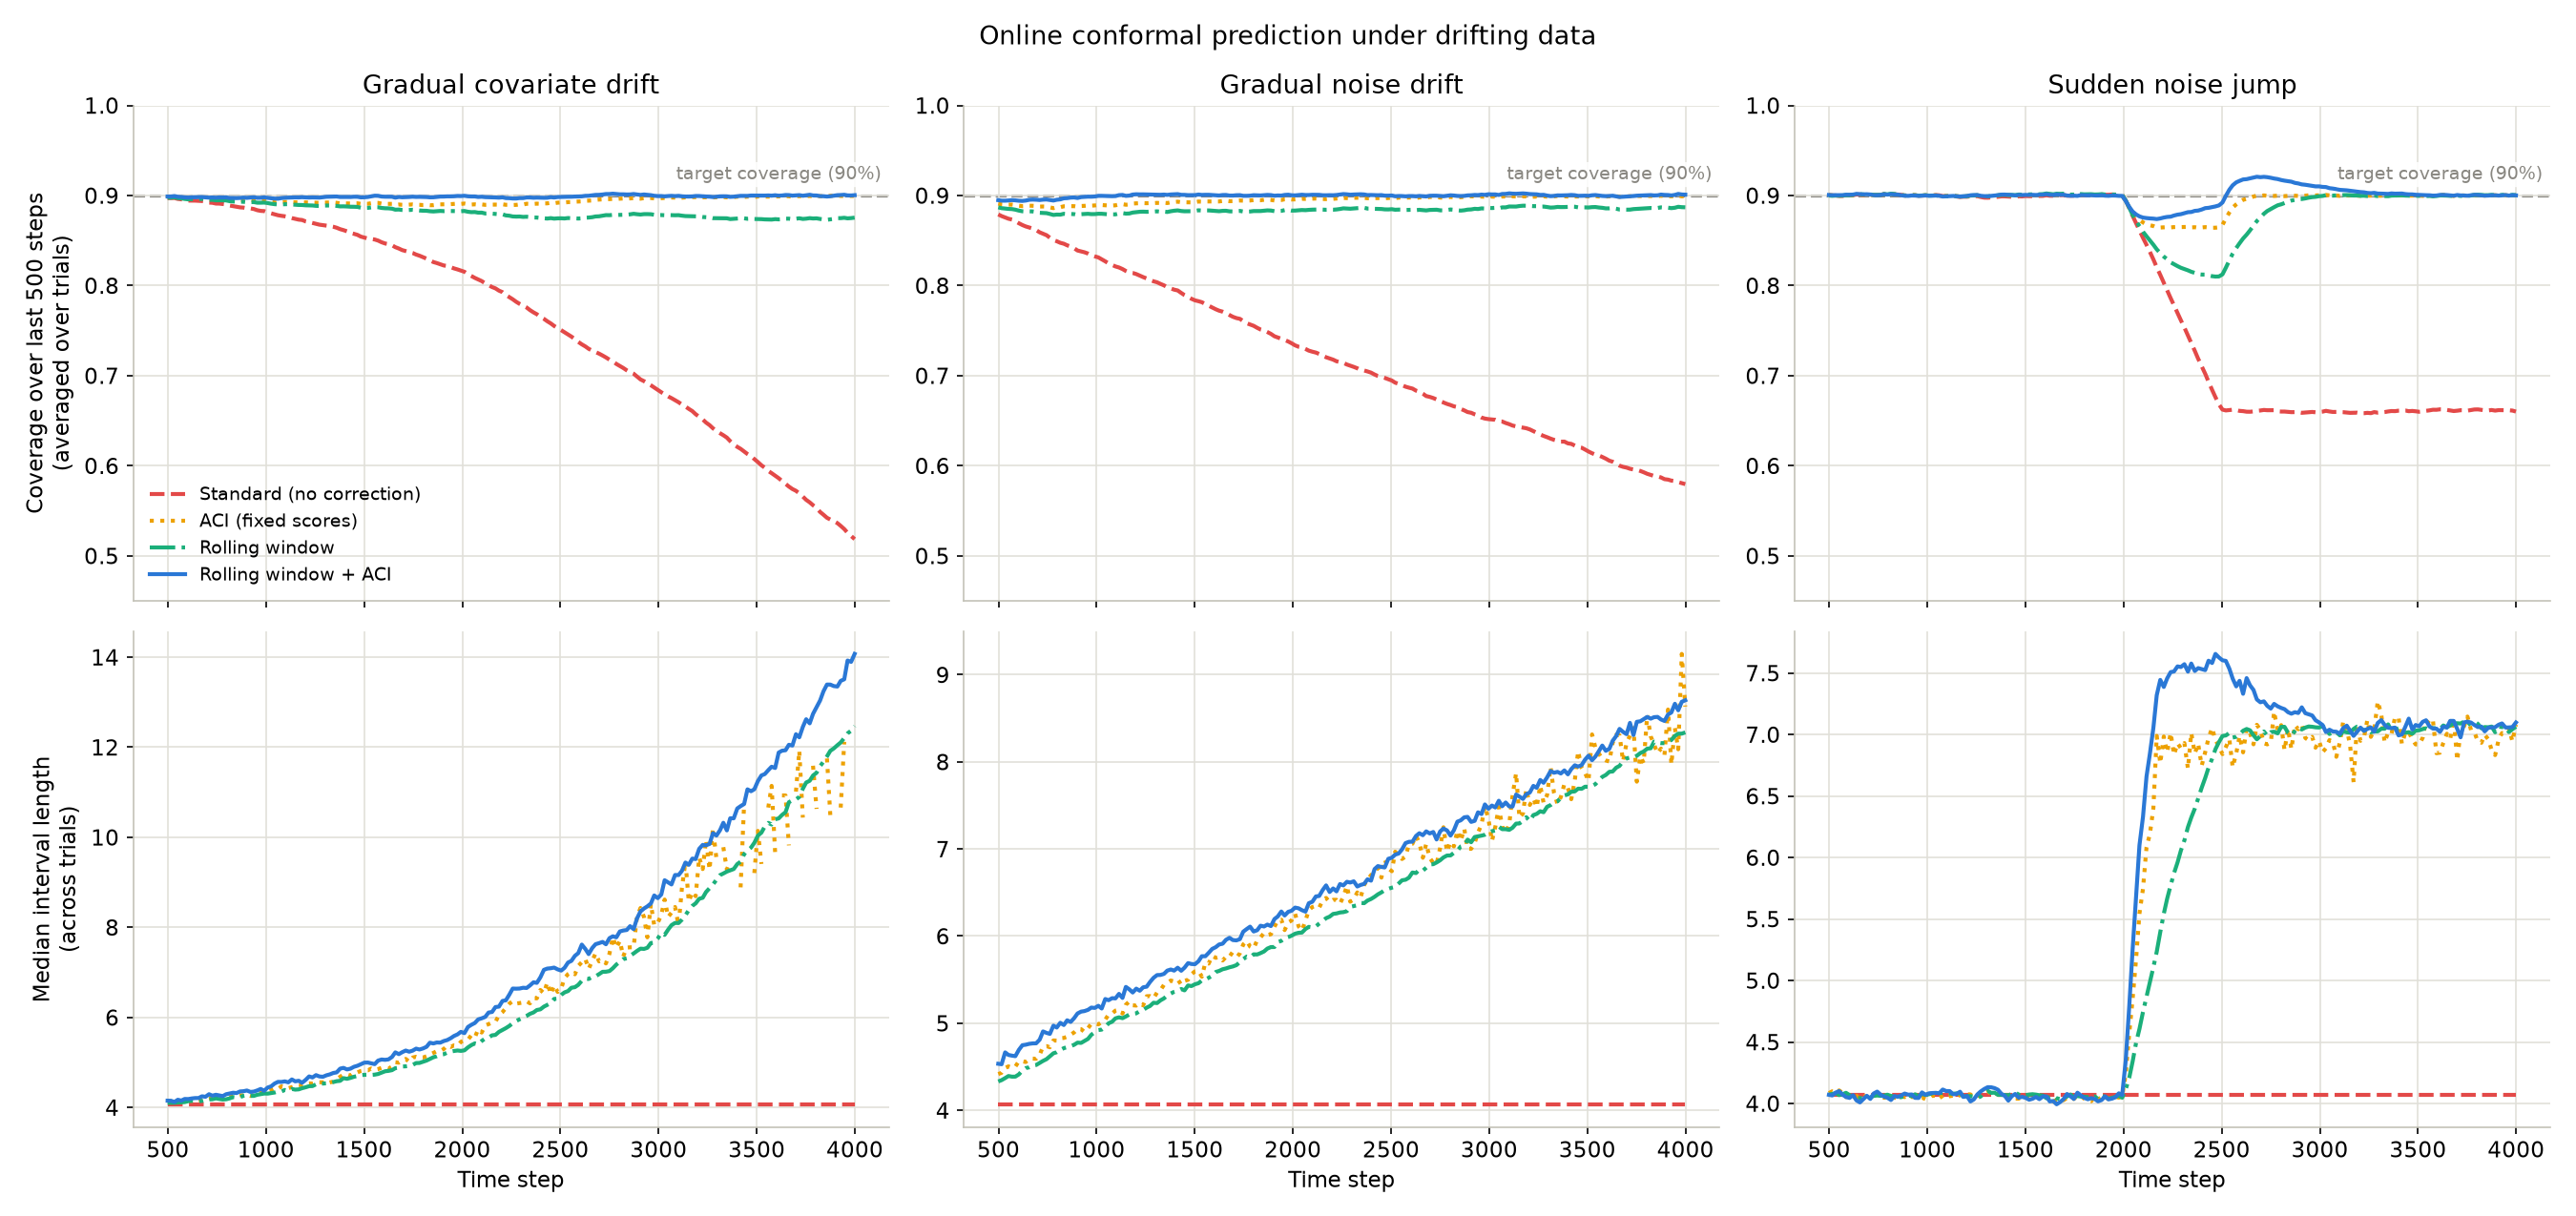
\includegraphics[width=\linewidth]{results/online.png}
  \caption{Top: coverage over the trailing 500 steps, averaged over 100 trials.
  Bottom: median interval length across trials at each step.}
  \label{fig:online}
\end{figure}

\begin{center}
\small
\begin{tabular}{ll rrrr}
\toprule
Scenario & Method & Long-run cov. & Worst local cov. & Median length & \% infinite \\
\midrule
Covariate drift & Standard & 75.1\% & 51.5\% & 4.07 & 0\% \\
 & ACI & 89.5\% & 87.4\% & 5.52 & 8.9\% \\
 & Rolling window & 88.3\% & 85.0\% & 5.28 & 0\% \\
 & Rolling + ACI & 89.9\% & 87.9\% & 5.78 & 0\% \\
\midrule
Noise drift & Standard & 72.2\% & 56.7\% & 4.07 & 0\% \\
 & ACI & 89.5\% & 87.4\% & 6.12 & 3.0\% \\
 & Rolling window & 88.5\% & 85.5\% & 6.00 & 0\% \\
 & Rolling + ACI & 90.0\% & 87.9\% & 6.27 & 0\% \\
\midrule
Noise jump & Standard & 78.0\% & 62.4\% & 4.07 & 0\% \\
 & ACI & 89.6\% & 85.6\% & 4.47 & 1.4\% \\
 & Rolling window & 88.9\% & 80.4\% & 4.35 & 0\% \\
 & Rolling + ACI & 90.0\% & 86.8\% & 4.62 & 0\% \\
\bottomrule
\end{tabular}
\end{center}

Without correction, coverage drifts steadily downward, reaching about 52\% by the
end of the covariate drift. All three online methods hold long-run coverage within
2 points of target, but they get there differently:

\begin{itemize}
  \item \textbf{ACI with fixed scores} meets its long-run guarantee (89.5--89.6\%,
    with a trial-to-trial sd below 0.05 points), but only by brute force. Once the
    required width exceeds the largest calibration residual, the only way to cover
    more is $\alpha_t \le 0$, an infinite interval. That happens on up to 8.9\% of
    steps under covariate drift. In the figure, this shows up as the jagged median
    length late in that stream.
  \item \textbf{A rolling window} keeps finite intervals by using recent residuals,
    but always \emph{lags}. Its scores describe the last 500 steps, not the present,
    so under gradual drift it sits 1.5--2.5 points below target throughout. After the
    sudden jump it falls to about 81\% for several hundred steps while the window
    fills with post-jump residuals.
  \item \textbf{Rolling window + ACI} is best on every measure: 89.9--90.0\%
    long-run coverage, the highest worst-case stretch in every scenario, and no
    infinite intervals. The two parts complement each other. The window keeps the
    scores on the right scale, and ACI corrects the window's remaining lag. After the
    sudden jump it briefly overshoots to about 92\%, as ACI works off the misses it
    accumulated during the transition, before settling back to 90\%.
\end{itemize}

\section{Results Summary}

\begin{enumerate}
  \item \textbf{Coverage must always be read next to interval width.} Every method
    that restores coverage does so by spending width. Recalibration widens intervals
    6.8-fold under large covariate shift, and weighted conformal returns infinite
    intervals for most points. A method that reports only coverage can look like it
    ``solved'' distribution shift while returning uselessly wide intervals.
  \item \textbf{Methods differ in \emph{where} they spend width.} Group-specific
    calibration and normalized scores widen intervals only for the points that are
    actually harder. They hold coverage under mixture-type shift at a far smaller
    cost than generic recalibration. This requires that the source of difficulty be
    observable, either as a known group label or as a function of $x$.
  \item \textbf{Validity without labels has limits set by overlap.} Weighted
    conformal is valid without any labels from the new distribution, and estimated
    weights work as well as exact ones here. But its usefulness decays with the
    effective sample size $n e^{-\|\mu\|^2}$. It is a tool for moderate shift, not
    extrapolation.
  \item \textbf{When labels arrive over time, online correction works.} ACI gives a
    long-run guarantee under arbitrary drift. Combined with a rolling calibration
    window, it holds 90\% coverage with finite intervals in every streaming
    scenario.
\end{enumerate}

\section{Limitations}
\label{sec:limitations}

\begin{itemize}
  \item All data are synthetic, from a single hand-chosen nonlinear function, and
    every shift is cleanly parameterized. Real distribution shift is rarely this
    tidy, and is often a combination of the shift types studied separately here.
  \item The covariate shift is a Gaussian mean shift, under which the true
    likelihood ratio is log-linear and logistic regression is correctly specified.
    Estimating weights for real, high-dimensional shifts is harder, so the near-perfect
    match between exact and estimated weights should not be expected in general.
  \item The recalibration fix assumes a fresh, labeled calibration set from the
    shifted distribution at the moment of shift, which real deployments rarely have.
  \item Group-specific calibration requires known group membership at both
    calibration and test time.
  \item The adaptive-interval experiment uses one heteroscedastic structure, driven
    by a single feature. Normalized scores benefit directly from how easy that
    structure is to learn, and the CQR results depend on untuned quantile models.
  \item The online experiments use one ACI step size ($\gamma = 0.005$) and one
    window length (500) without tuning. The base model is never retrained, and
    stream points are independent given time, with no autocorrelation. Labels are
    assumed to arrive immediately after each prediction.
  \item Base models use largely default hyperparameters; absolute width numbers (not
    the qualitative trends) would change with more carefully tuned models.
\end{itemize}

\section{Future Work}

\begin{itemize}
  \item Move from synthetic data to a real dataset with a natural shift (e.g.\ a
    temporal or geographic split), to check whether these findings transfer.
  \item Explore subgroup-shift robustness when group labels are \emph{not} known,
    e.g.\ by clustering residuals or covariates to discover latent subgroups before
    calibrating per cluster.
  \item Combine methods: normalized scores inside weighted conformal or ACI, so
    intervals adapt both to local difficulty and to shift.
  \item Remove the need to hand-pick ACI's step size, e.g.\ by running several
    step sizes in parallel and adaptively choosing among them, and study delayed
    labels and periodic model retraining in the streaming setting.
  \item Add diagnostics for weighted conformal, such as reporting the effective sample
    size, so a deployed system can flag when the calibration data no longer cover the
    test distribution, instead of silently returning infinite intervals.
\end{itemize}

\section*{References}

\begin{itemize}
  \item Gibbs, I.\ and Cand\`es, E.\ (2021). Adaptive conformal inference under
    distribution shift. \emph{Advances in Neural Information Processing Systems 34}.
  \item Lei, J., G'Sell, M., Rinaldo, A., Tibshirani, R.\ J.\ and Wasserman, L.\
    (2018). Distribution-free predictive inference for regression. \emph{Journal of
    the American Statistical Association}, 113(523), 1094--1111.
  \item Papadopoulos, H., Proedrou, K., Vovk, V.\ and Gammerman, A.\ (2002).
    Inductive confidence machines for regression. \emph{Proceedings of the 13th
    European Conference on Machine Learning (ECML)}, 345--356.
  \item Romano, Y., Patterson, E.\ and Cand\`es, E.\ (2019). Conformalized quantile
    regression. \emph{Advances in Neural Information Processing Systems 32}.
  \item Tibshirani, R.\ J., Barber, R.\ F., Cand\`es, E.\ and Ramdas, A.\ (2019).
    Conformal prediction under covariate shift. \emph{Advances in Neural Information
    Processing Systems 32}.
\end{itemize}

\end{document}
